\chapter{Must Have Concepts}
\label{chapter:must_have_concepts}
During this chapter, the author will discuss topics that help understand the technological developments along this thesis project. The developments will involve both hardware and software components. As such, there are hardware and software concepts that are important to have before discussing the following chapters.

The candidate will develop a \acrshort{soc} in this project. However, he will not create it from scratch. The candidate will use the \textit{IOb-SoC} as a starting point. Consequently, it is important to understand how the \textit{IOb-SoC} works beforehand. It is also important to study the \textit{RISC-V} \acrfull{isa}. Since the hardware developed in this project will be compatible with the \textit{RISC-V} \acrshort{isa}. Furthermore, the software developed will be cross-compiled with the \textit{RISC-V} toolchain. An important part when developing a system is its testing and simulation before implementation. Therefore, the author will review the available methods for simulating the developed components. Lastly, an important concept for this project is the boot flow of an \acrfull{os} on a \textit{RISC-V} platform.

\section{The \textit{IOb-SoC} platform}
\label{section:iob_soc_template}
The \textit{IOb-SoC}~\cite{iob_soc} is a \acrfull{soc} template that eases the creation of a new SoC. The \textit{IOb-SoC} provides a base Verilog~\cite{thomas2008verilog} hardware design equipped with an open-source \textit{RISC-V} processor, an internal SRAM memory subsystem, a \acrshort{uart}, and an optional interface to external memory. If the external memory interface is selected, the \textit{IOb-SoC} will include an instruction L1 cache, a data L1 cache and a shared L2 cache. The L2 cache communicates with a third-party memory controller IP (typically a \acrshort{ddr} controller) using an AXI4~\cite{tidala2018high} master bus. Users can add IP cores and software to build their own SoCs quickly. This way, hardware accelerators can be easily created and tested with the developed firmware.

In figure \ref{fig:bd_original} it is represented a sketch of the \acrshort{soc} design. This design is valid at the start of this project. During the hardware developed chapter \ref{chapter:hardware_developed} some alterations were made to the \textit{IOb-SoC} original template.

\begin{figure}[!h]
    \centering
    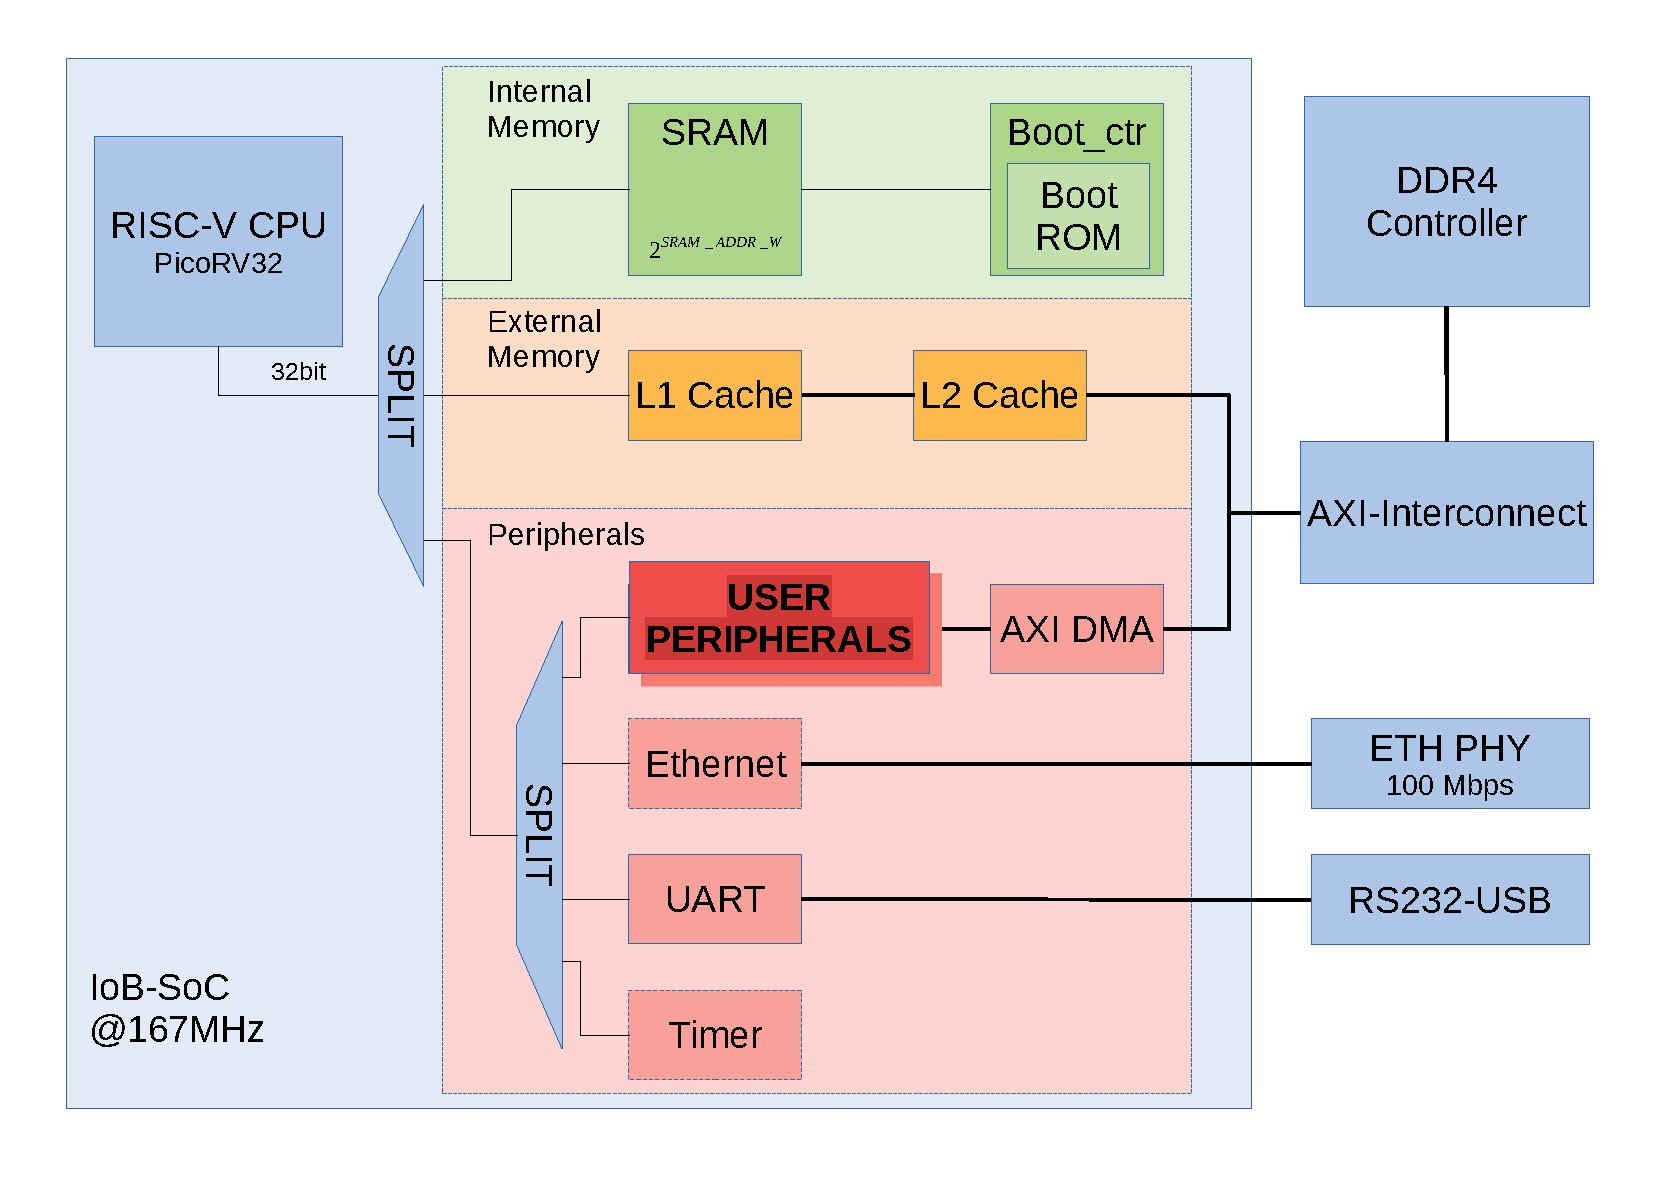
\includegraphics[width=0.7\linewidth]{bd_original.pdf}
    \caption{\textit{IOb-SoC} sketch.}
    \label{fig:bd_original}
\end{figure}

Building a new processor-based system from scratch can be difficult. The \textit{IObundle} developers created the \textit{IOb-SoC} to facilitate this process. This work develops a variant of the existing \textit{IOb-SoC} capable of running a Linux Operating System. \textit{IOb-SoC} currently supports two FPGA board models: the Xilinx Kintex UltraScale KU040 Development Board and the Cyclone V GT FPGA Development Kit.

\subsection{\textit{IOb-SoC} \textit{Makefiles}}
\label{subsection:iob_makefiles}
\textit{Makefiles} are essential because they allow automating processes. This way, instead of executing multiple lines to achieve a goal, the user can run a single command. That command will execute a \textit{Makefile} script that runs the multiple processes needed to achieve a specific goal without specifying them. For example, to run a simulation, a developer using this project \acrshort{soc} would only have to write in the terminal the commands in listing~\ref{lst:run_simulation}.

\begin{lstlisting}[language=make, caption={Run a simulation.}, label=lst:run_simulation]
    make sim-clean
    make sim-run
\end{lstlisting}

The first command in listing~\ref{lst:run_simulation} cleans all the files related to a previous simulation execution. Then the second command runs a new simulation. This simulation will use the default configurations in the \enquote{config.mk} file. A \textit{Makefile} target follows each of the \enquote{make} commands. A target is a section of the \textit{Makefile} that may or may not depend on other targets and executes a sequence of commands. In the example~\ref{lst:run_simulation} there are two targets, \enquote{sim-clean} and \enquote{sim-run}.

The main \textit{Makefile} in \textit{IOb-SoC} is located at the \textit{IOb-SoC} root directory. The main \textit{Makefile} contains targets that call other \textit{Makefiles} and sets the values for the default frequency, baud rate, \acrshort{fpga} board used and simulator used. The \textit{Makefiles} the main one can call are at the \textit{IOb-SoC} \acrshort{fpga} boards, simulators, firmware, \enquote{PC} emulation or documentation directory. Each directory in \textit{IOb-SoC} contains a \enquote{*.mk} file which holds \enquote{make} variables and targets that complement the \textit{Makefiles}. The \textit{IOb-SoC} \textit{Makefiles} can include only the \enquote{*.mk} they need.

When executing the command \lstinline[language=bash]{make sim-run} the computer will run the \enquote{run} target of the \textit{Makefile} in the default simulator directory. The simulator \textit{Makefile} will include the \enquote{simulator.mk}, \enquote{hardware.mk} and \enquote{config.mk} files. The \enquote{simulator.mk} file is common to all simulators. Both \acrshort{fpga}s and simulators \textit{Makefiles} include the \enquote{hardware.mk} file. The \enquote{hardware.mk} file includes all the hardware modules that the \acrshort{soc} uses. Lastly, the \enquote{config.mk} is located at the \textit{IOb-SoC} root directory and all \textit{Makefiles} use it. The \enquote{config.mk} defines the \enquote{make} variables that are important for hardware and software, for example which peripherals the \acrshort{soc} contains.

\subsection{\textit{IOb-SoC} peripherals}
\label{subsection:iob_peripherals}
Developers add the \textit{IOb-SoC} peripherals under the submodules directory in the \textit{IOb-SoC} folder. Inside the submodules directory, there exists a folder for each peripheral. Furthermore, the \acrshort{cpu}, the \enquote{iob\_cache} module, the \enquote{iob\_mem} hardware, the \enquote{iob\_axi} interface and the \textit{IOb-Lib}~\cite{iob_lib} repository can also be found in the submodules directory. The \textit{IObundle} engineers developed the \textit{IOb-Lib} submodule for it to contain small generic hardware modules and software script used in \textit{IOb-SoC}.

All the submodules may contain hardware and software components. For each hardware peripheral, the \textit{IOb-SoC} engineers recommend developing a set of bare-metal firmware functions that allow using the peripheral with the \acrshort{soc} without an \acrshort{os}. Since the \textit{IOb-SoC} platform also allows emulating the developed firmware in the user's personal computer, the peripherals should have software functions that emulate its firmware drivers.

The peripheral should have the following \enquote{*.mk} files to integrate it into \textit{IOb-SoC}:
\begin{itemize}
    \item the \enquote{PERIPHERAL\_REPO/hardware/hardware.mk} so the user can add the peripheral hardware modules to the \acrshort{soc}.
    \item the \enquote{PERIPHERAL\_REPO/software/embedded/embedded.mk} allows the user to use the peripheral firmware drivers.
    \item the \enquote{PERIPHERAL\_REPO/software/pc-emul/pc-emul.mk} permits emulating the peripheral behaviour in the user's computer.
\end{itemize}
The developer has to include the \enquote{PERIPHERAL\_REPO/hardware/hardware.mk} file in the \textit{IOb-SoC} \enquote{hardware.mk} file. He can include it by adding \lstinline[language=make]{include $(PERIPHERAL_DIR)/hardware/hardware.mk} to the \textit{IOb-SoC} \enquote{hardware.mk}. In the firmware \textit{Makefile} the develops has to include the peripherals \enquote{embedded.mk} file by adding \lstinline[language=make]{include $(PERIPHERAL_DIR)/software/embedded/embedded.mk} to use the peripheral drivers. Lastly in the \enquote{pc-emul} \textit{Makefile} he has to add \lstinline[language=make]{include $(PERIPHERAL_DIR)/software/pc-emul/pc-emul.mk} to allow the software to emulate the peripheral.

In the \enquote{config.mk} file, located in the \textit{IOb-SoC} repository root, the developer needs to add the \enquote{PERIPHERAL\_REPO} to the \enquote{PERIPHERALS} \enquote{make} variable and create a variable that indicates the peripheral directory. The user should define the variable that indicates the peripheral directory similarly to \lstinline[language=make]{PERIPHERAL_DIR=$(ROOT_DIR)/submodules/PERIPHERAL_REPO}.

The peripheral also needs the following files to be automatically instantiated in the \acrshort{soc} hardware: \enquote{inst\_tb.vh}, \enquote{inst.vh} and \enquote{pio.vh}. The \textit{Makefiles} use the \enquote{inst\_tb.vh} file to add the needed Verilog to the testbench core for the system to simulate. It uses the \enquote{inst.vh} to instantiate the peripheral hardware module in the \textit{IOb-SoC} core. Finally, the \enquote{pio.vh} file contains input and output signals that the \textit{Makefiles} must add to the system core hardware. Those files should be in the \enquote{PERIPHERAL\_REPO/hardware/include} directory. Listing \ref{lst:inst_file} presents an example of the \enquote{inst.vh} contents.

\begin{lstlisting}[language=Verilog, caption={Example of the \enquote{inst.vh} file.}, label=lst:inst_file]
//
// TIMER
//
iob_timer timer
  (
   .clk      (clk),
   .rst      (reset),

   //cpu interface
   .valid(slaves_req[`valid(`TIMER)]),
   .address(slaves_req[`address(`TIMER,`TIMER_ADDR_W+2)-2]),
   .wdata(slaves_req[`wdata(`TIMER)]),
   .wstrb(slaves_req[`wstrb(`TIMER)]),
   .rdata(slaves_resp[`rdata(`TIMER)]),
   .ready(slaves_resp[`ready(`TIMER)])
   );
\end{lstlisting}

\subsection{Internal Buses}
\label{subsection:iob_bus}
The \textit{IObundle} developers designed the \textit{IOb-SoC} in a way that one master hardware component and multiple slave hardware components exist. To Interconnect the hardware components \textit{IOb-SoC} defines two types of bus, the request bus and the response bus. In \textit{IOb-SoC} the master component is the \acrshort{cpu}. The \acrshort{cpu} sends requests to the internal or external memory and the peripherals through the request buses. After making a request, the \acrshort{cpu} will receive the response through the respective response bus. The \acrshort{cpu} instantiated in the \textit{IOb-SoC} core has the \enquote{cpu\_i\_req}, \enquote{cpu\_d\_req}, \enquote{cpu\_i\_resp} and \enquote{cpu\_d\_resp} signals. The \enquote{cpu\_i\_req} signal serves to fetch instructions from memory, and the \enquote{cpu\_i\_resp} will contain the instruction fetched after a few clock cycles. The \acrshort{cpu} uses the \enquote{cpu\_d\_req} to make data requests to either the memory or a \acrshort{soc} peripheral.

The request bus comprises a valid bit, an address signal, a data signal and a strobe signal. The hardware sets the valid bit to ‘1’ when it wants to execute a request and has already defined the other signals. The address signal indicates the register that the request is targeting. Figure \ref{fig:req_bus} shows how the \textit{IOb-SoC} distributes the signals in the request bus. Furthermore, figure \ref{fig:req_bus} also represents the bits equivalent to each signal when the address width and data width are 32 bits. The address and data width in \textit{IOb-SoC} are 32-bit by default.

\begin{figure}[!h]
    \centering
    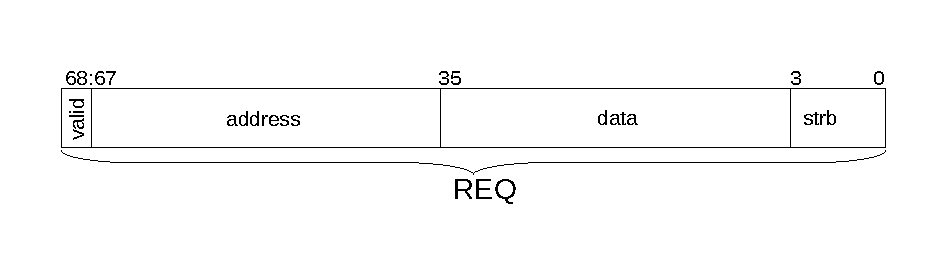
\includegraphics[width=\linewidth]{req_bus.pdf}
    \caption{Request bus with address and data width equal to 32 bits.}
    \label{fig:req_bus}
\end{figure}

The response bus contains a ready bit and a data signal. The hardware sets the ready signal to high when the component that made the request can receive the response. The data signal is the response data to the request made. For example, if the \acrshort{cpu} wants to read the value in a register at address \enquote{x}, the data in the response bus will be the data on register \enquote{x}. Figure \ref{fig:resp_bus} shows how the request signal is composed when the address and data width are 32 bits.

\begin{figure}[!h]
    \centering
    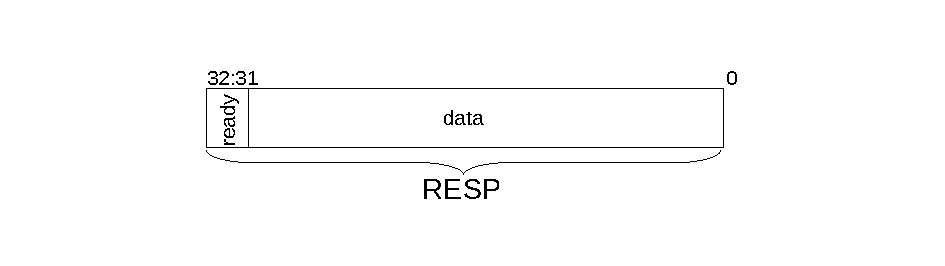
\includegraphics[width=\linewidth]{resp_bus.pdf}
    \caption{Response bus with address and data width equal to 32 bits.}
    \label{fig:resp_bus}
\end{figure}

In the \textit{IOb-Lib} submodule exists a file, called \enquote{iob\_intercon.vh}, that defines a set of macros that can be used in \textit{Verilog}. Developers can use those macros to access the specific bits in the \textit{IOb-SoC} buses. Table \ref{tab:bus_defines} shows the defined macros, how the pre-compiler calculates their value and the respective values when the address and data width are 32-bit.

\begin{table}[!ht]
    \centering
    \resizebox{\textwidth}{!}{%
    \begin{tabular}{|l|l|l|l|}
    \hline
    \textbf{Name} & \textbf{Defined expression}          & \textbf{Description}                  & \textbf{\begin{tabular}[c]{@{}l@{}}Value with:\\   ADDR\_W=32\\   DATA\_W=32\end{tabular}} \\ \hline
    READY\_W      & 1                                    & Response ready width                  & 1                                                                                          \\ \hline
    VALID\_W      & 1                                    & Request valid width                   & 1                                                                                          \\ \hline
    WSTRB\_W      & DATA\_W/8                            & Request data width                    & 4                                                                                          \\ \hline
    WRITE\_W      & DATA\_W+DATA\_W/8                    & Most significant bit of request data  & 36                                                                                         \\ \hline
    READ\_W       & DATA\_W+READY\_W                     & Most significant bit of response data & 33                                                                                         \\ \hline
    WDATA\_P      & DATA\_W/8                            & Less significant bit of request data  & 4                                                                                          \\ \hline
    ADDR\_P       & DATA\_W+DATA\_W/8                    & Less significant bit of request data  & 36                                                                                         \\ \hline
    VALID\_P      & ADDR\_W+DATA\_W+DATA\_W/8            & Request bus valid bit position        & 67                                                                                         \\ \hline
    REQ\_W        & VALID\_W+ADDR\_W+WRITE\_W            & Request bus width                     & 69                                                                                         \\ \hline
    RESP\_W       & DATA\_W+READY\_W                     & Response bus width                    & 33                                                                                         \\ \hline
    req(I)        & I*REQ\_W +: REQ\_W                   & Request bus bits boundary             & I*69 +: 69                                                                                 \\ \hline
    resp(I)       & I*RESP\_W +: RESP\_W                 & Response bus bits boundary            & I*33 +: 33                                                                                 \\ \hline
    valid(I)      & I*REQ\_W+VALID\_P                    & Request valid bit position            & I*69+1                                                                                     \\ \hline
    address(I,W)  & I*REQ\_W+ADDR\_P+W-1 -: W            & Request address bits boundary         & I*69+W+35 -: W                                                                             \\ \hline
    wdata(I)      & I*REQ\_W+WDATA\_P +: DATA\_W         & Request data bits boundary            & I*69+4 +: 32                                                                               \\ \hline
    wstrb(I)      & I*REQ\_W +: WSTRB\_W                 & Request strb bits boundary            & I*69 +: 4                                                                                  \\ \hline
    write(I)      & I*REQ\_W +: WRITE\_W                 & Request write bits boundary           & I*69 +: 36                                                                                 \\ \hline
    rdata(I)      & I*RESP\_W+READY\_W +: DATA\_W        & Response data bits boundary           & I*33+1 +: 32                                                                               \\ \hline
    ready(I)      & I*RESP\_W                            & Response ready bit position           & I*33                                                                                       \\ \hline
    \end{tabular}
    }
    \caption{Bus interconnect macros.}
    \label{tab:bus_defines}
\end{table}

Understanding the interconnect macros is essential when developing the interface with peripherals and hardware components for the \textit{IOb-SoC}. Some macros depend on an \enquote{I} value given to them when using the macro. The hardware uses the  \enquote{I} value to distinguish which request or response signal the developers want to access when there is a bus (i.e. wire) with multiple requests or responses. In the \enquote{address(I,W)} macro, the \enquote{W} value corresponds to the number of bits of the address in the request signal the developer wants to select.

\subsection{\textit{iob-split} and \textit{iob-merge}}
\label{subsection:iob_split_merge}
The \textit{iob-split} and the \textit{iob-merge} hardware modules can both be found in the \textit{IOb-Lib} submodule hardware directory. The \textit{IOb-SoC} uses the \textit{iob-split} in the systems core and in the internal memory hardware modules. The \textit{iob-split} in \textit{IOb-SoC} separates one request and one response bus into multiple buses and only enables the needed one. For example, there are multiple peripherals; each has an input request bus and an output response bus. However, there is only one \enquote{cpu\_d\_req}. The \textit{iob-split} only sends the \enquote{cpu\_d\_req} signal to the selected peripheral and sets the other peripherals request bus to zeros. The \textit{IOb-SoC} instantiates the \textit{iob-merge} in the external and internal memory hardware modules. The \textit{iob-merge} unifies multiple request and response buses into one. For example, the \acrshort{cpu} can execute both instructions and data requests to the memory. Nevertheless, the memory can only process one request at a time. The \textit{iob-merge} merges the \enquote{cpu\_i\_req} and the \enquote{cpu\_i\_req} and sends to the memory the request with higher priority or the one that was first set has valid.

The \textbf{\textit{iob-split}} is simply a configurable \acrfull{demux}. The developer can configure it when he instantiates the \textit{iob-split} hardware module. The developer can change the size of the \acrlong{demux} and the selection bits through N\_SLAVES and P\_SLAVES, respectively. N\_SLAVES corresponds to the number of slaves. Developers can also interpret N\_SLAVES as the number of the \acrshort{demux} outputs. P\_SLAVES indicates the slave select word \acrfull{msb} position. In other words, P\_SLAVES is the position of the \acrshort{msb} of the \acrlong{demux} selection bits. Equation \ref{eq:number_bits} calculates the number of the selection bits.

\begin{equation}
    \label{eq:number_bits}
    Nb = log_2(N\_SLAVES)+(log_2(N\_SLAVES)==0)
\end{equation}

The \textbf{\textit{iob-merge}} works similar to the \textit{iob-split} but instead of being a \acrshort{demux} it is a configurable \acrfull{mux}. Meaning that instead of having multiple outputs and one input, it has multiple inputs and one output. N\_SLAVES indicates the number of inputs, and P\_SLAVES chooses the selection bits.

\subsection{Bootloader}
The \textit{IObundle} engineers developed a bootloader for \textit{IOb-SoC} that is the first firmware to run on the \acrlong{soc}. The \textit{IOb-SoC} always saves the bootloader firmware in the \acrshort{soc} internal memory in a boot control hardware unit. The boot control hardware unit defines the boot signal. The boot signal is one bit that can be set to high ('1') or low ('0') and indicates whether the \acrshort{soc} should execute the bootloader or other firmware. Moreover, the boot control unit sends a reset signal to the \acrshort{cpu} when the bootloader ends before starting the users' firmware.

Figure \ref{fig:boot_flow} represents a flow chart of the bootloader firmware behaviour. The bootloader starts by initialising the \acrshort{uart} hardware which the \acrshort{soc} uses to communicate with the user's computer. Then it will send an \acrfull{enq} if it still has not sent one. The \acrshort{enq} byte has the value of 0x05 in \acrshort{ascii} and is sent to the user's computer to indicate that the \textit{IOb-SoC} is waiting for the user's computer. The bootloader will ensure the \acrshort{uart} is sending the \acrshort{enq} byte while the user's computer does not send a response. After receiving a response byte, the bootloader firmware checks if the received byte is an \acrfull{frx}. The \acrshort{frx} Byte has the value 0x07. If the bootloader receives a \acrshort{frx}, it has to transfer the firmware that runs after it.

\begin{figure}[!h]
    \centering
    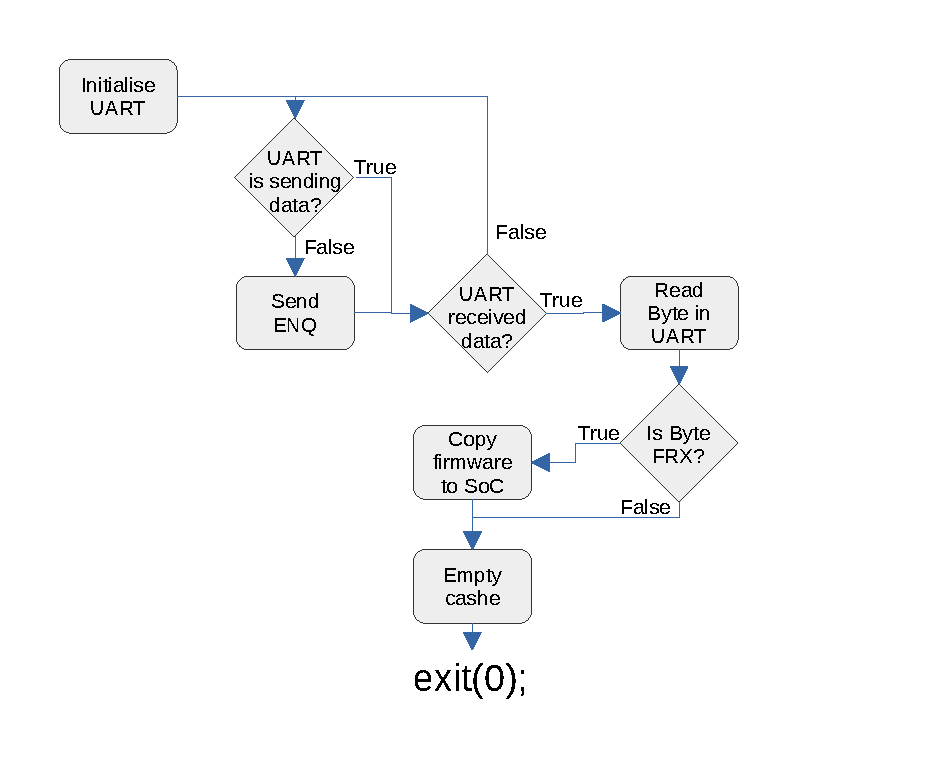
\includegraphics[width=\linewidth]{boot_flow.pdf}
    \caption{Bootloader firmware flow chart.}
    \label{fig:boot_flow}
\end{figure}

When transferring the firmware, the bootloader receives the binary data through the \acrshort{uart} and copies it to the \acrshort{soc} memory. The bootloader can copy the firmware to either the internal or external memory depending on where the user defined the program would be stored. After copying the firmware to the \textit{IOb-SoC}, the bootloader will send the data saved in the memory back to the user's computer. The user's computer can then check if the \textit{IOb-SoC} successfully transferred the firmware by comparing the original firmware binary with the received copy. Before exiting, the bootloader will clean the cache so that the next firmware does not fetch data previously in the cache. Finally, when exiting, the bootloader asks the boot control unit to set the boot signal to low and reset the \acrshort{cpu}.

\section{\textit{RISC-V}}
\label{section:riscv}
\textit{RISC-V}~\cite{asanovic2014instruction} is a free, open-source RISC Instruction Set Architecture (ISA). An ISA is the bridge that connects software and hardware. RISC is one possible classification of the computer ISA's; it means reduced instruction set computer, and the essence of this approach is the simplicity of the instructions computed by the CPU. Unlike a Complex Instruction Set Computer (CISC) ISA, the CPU might have to execute a more significant number of instructions with a RISC ISA to obtain the same result. Since the instructions are simple, more instructions need to be run to complete a given task. However, the architecture is lighter and can run at a higher frequency, compensating for executing more instructions.

The \textit{RISC-V} was initially designed at the University of California, Berkeley. Furthermore, it is called \textit{RISC-V} because it is the fifth RISC instruction set architecture to come out of that university. It was created to support computer architecture research and education. Although now \textit{RISC-V} is used on commercial projects as well. A key advantage of \textit{RISC-V} is its flexibility. It can be used from high-performance computers to deeply embedded systems with no MMU. There exists a 32, 64 and 128-bit version of \textit{RISC-V}. In this report, the 32 and 64-bit versions will be discussed. On the work developed during the thesis preferentially, the 32-bit version will be used. If an instruction is not on the standard \textit{RISC-V}, it can be created as an ISA extension, which provides excellent flexibility.

There are two main parts of the \textit{RISC-V} ISA. There are the \textit{unprivileged} instructions that correspond to the base ISA~\cite{riscv_unpriviledge}, which is composed of only 32-bit instructions and some unprivileged extensions. {Unprivileged instructions} are the instructions that can be used on all privilege modes in all privilege architecture. Moreover, there exists the privilege instructions~\cite{riscv_priviledge} that implements support for the three different privilege levels. Machine mode is the most trusted privilege level, and typically what runs in this mode has low-level access to the machine implementation. The other two modes are the User mode, where most common applications run, and the OS's Supervisor mode. Each privileged mode has its extensions to the ISA.

What a Hart is???

Developers need the \textit{RISC-V} toolchain to cross-compile software for \textit{RISC-V} platforms. The \textit{RISC-V} foundation makes the toolchain available for download in their github page. The \textit{RISC-V} toolchain has two main types of the cross-compilers the Newlib and the Linux version. Furthermore developers can install the toolchain to work with 32-bit, 64-bit or both system architectures. The author installed the Newlib and the Linux \textit{RISC-V} toolchain with multilib (i.e. support for both 32-bit and 64-bit architecture). The \textit{IOb-SoC} uses the Newlib cross-compiler to compile firmware to run in bare-metal. Developers need to compile the linux kernel and software related to the \acrshort{os} with the Linux cross-compiler.

The \textit{RISC-V} specification defines that a \acrshort{cpu} compatible with \textit{RISC-V} has to have thirty two internal registers. Those registers width is equal to the architecture bit width, it could be 32-bit, 64-bit or 128-bit. The table \ref{tab:riscv_cpu_registers} in annex \ref{appendix:riscv_cpu_regs} presents the 32 registers a \textit{RISC-V} \acrshort{cpu} has.


\subsection{ISA extensions}
\label{subsection:isa_extensions}
The instruction each ISA extension contains...

\subsection{Control Status Registers}
\label{subsection:csr}
\acrfull{csr} needed to run a full feature OS... (core\_id, misa, mcause, ...)

\subsection{Compatible CLINT}
\label{subsection:clint_riscv}
The \textit{RISC-V} \acrshort{clint} specification~\cite{clint_riscv_spec} describes the hardware registers of a \acrfull{clint} compatible with \textit{RISC-V} platforms. The hardware uses the \acrshort{clint} to generate the inter-processor software and timer interrupts. \textit{SiFive} developed their Core-Local Interrupt (CLINT) device before the \textit{RISC-V} foundation made the \acrshort{clint} specification. Therefore, the RISC-V community has widely adopted it in their projects.

Table \ref{tab:clint_spec_regs} shows the \acrshort{clint} registers compatible with the \textit{SiFive} \acrshort{clint} and the \textit{RISC-V} specification. The \acrshort{clint} implemented in this thesis project only uses machine-level interrupts. However, the \textit{RISC-V} \acrshort{clint} specification also specifies the supervisor inter-processor software interrupts, which the author does not approach here.

\begin{table}[!ht]
    \centering
    \begin{tabular}{|l|l|l|l|l|}
    \hline
    \textbf{Name} & \textbf{Address} & \textbf{Width (bit)} & \textbf{Access} & \textbf{Description}                                                                  \\ \hline
    MSIP0         & 0x0              & 32                   & RW              & HART index 0 machine-level IPI register                                               \\ \hline
    MSIP1         & 0x4              & 32                   & RW              & HART index 1 machine-level IPI register                                               \\ \hline
    ...           & ...              & ...                  & ...             & ...                                                                                   \\ \hline
    RESERVED      & 0x3FFC           & 32                   & -               & Reserved for future use.                                                              \\ \hline
    MTIMECMP0     & 0x4000           & 64                   & RW              & HART index 0 machine-level time compare                                               \\ \hline
    MTIMECMP1     & 0x4000           & 64                   & RW              & HART index 1 machine-level time compare                                               \\ \hline
    ...           & ...              & ...                  & ...             & ...                                                                                   \\ \hline
    MTIMECMP4094  & 0x7FF0           & 64                   & RW              & \begin{tabular}[c]{@{}l@{}}HART index 4094 machine-level time\\  compare\end{tabular} \\ \hline
    MTIME         & 0xbff8           & 64                   & RW              & Machine-level time counter                                                            \\ \hline
    \end{tabular}
    \caption{\acrshort{clint} registers compatible with \textit{SiFive} and the \textit{RISC-V} specification.}
    \label{tab:clint_spec_regs}
\end{table}

Each \textit{RISC-V} Hart should be connected to an \enquote{msip} and \enquote{mtip} pin in the \acrshort{clint} hardware unit. Through those pins, the \acrshort{clint} will notify the \acrshort{cpu} when software or timer interrupt occurs. Each \enquote{msip} pin is hardwired to the \acrshort{lsb} of the corresponding \enquote{MSIP} register. The value stored in the \enquote{MSIP} register must be '0' after the hardware resets the \acrshort{clint}. The only way the \enquote{MSIP} register value changes is if the \acrshort{cpu} writes to it. The \acrshort{cpu} is only able to write either '0' or '1' to the \enquote{MSIP} register. The 31 \acrshort{msb} of the \enquote{MSIP} can be hardwired to '0' and only the \acrshort{lsb} changes value.

The \enquote{mtip} pins are connected to the output of a digital comparator with the respective \enquote{MTIMECMP} register and the \enquote{MTIME} register as input. A digital comparator is a hardware component that takes two numbers as input in binary form and determines whether one number is greater than, less than or equal to the other. The \enquote{mtip} triggers when the \enquote{MTIMECMP} register value is lower then the \enquote{MTIME} register. On \acrshort{clint} reset, the hardware has to set the \enquote{MTIME} register value to '0', and the \enquote{MTIMECMP} register to a value that does not trigger the timer interrupt, for example, all bits set to '1'. Moreover, the \acrshort{clint} timer counter resolution must be 100ns or less (corresponding to a clock tick frequency of at least 10 MHz).

\subsection{Compatible PLIC}
\label{subsection:plic_riscv}
The \textit{RISC-V} systems use the \acrfull{plic} hardware to gather various device interrupts and have only one external interrupt line per \textit{RISC-V} Hart context. A \acrshort{plic} that claims to be a PLIC-Compliant standard \acrshort{plic} has to follow the \textit{RISC-V} \acrshort{plic} specification~\cite{plic_riscv_spec}. The \textit{RISC-V} \acrshort{plic} was first described in the privilege instructions documentation. Since version 1.10, the \textit{RISC-V} foundation has moved the \acrshort{plic} specification to its documentation. However, nothing major has changed, and \acrshort{plic} cores compatible with the \acrshort{plic} described in the privilege documentation are still compatible with the current standard.

The \acrshort{plic} hardware has many features that the author will not discuss here. In this thesis project, the author adapted an already developed \acrshort{plic} core to his work. To integrate an existing \acrshort{plic} core, what is essential to understand is how the system handles interrupt notifications and the \acrshort{plic} memory-mapped registers. Furthermore, each interrupts pin of a hardware peripheral connected to the \acrshort{plic} unit corresponds to a source. Additionally, a \textit{RISC-V} Hart connected to the \acrshort{plic} has to have at least one external interrupt pin. The \acrshort{plic} considers each external interrupt pin as a target. The \acrshort{plic} notifies the \acrshort{cpu} of an existing interrupt through the target signal connected to the \acrshort{cpu} external interrupt pin. A \textit{RISC-V} Hart can have one external interrupt input for \acrlong{machine} level interrupts and another for \acrlong{supervisor} level interrupts.

Figure \ref{fig:plic_int_flow} was obtained from the \textit{RISC-V} \acrshort{plic} specification and shows a sketch of the interrupt flow between the \acrshort{plic} hardware and the \acrshort{cpu}. When a peripheral generates an interrupt, the corresponding source input in the \acrshort{plic} is enabled, and the \acrshort{plic} forwards it to the interrupt gateway that processes the interrupt signal from each source. Then the interrupt gateway sends a single interrupt request to the \acrshort{plic} core, which latches these in the core interrupt pending bits (IP). Afterwards, the \acrshort{plic} core will send a notification to the targets to whom the interrupt interests. When a target receives an interrupt notification, it sends a claim request to the \acrshort{plic} core and waits for the response, which contains the interrupt id. After sending the identifier of the highest priority global interrupt source pending for that target, the \acrshort{plic} core clears the corresponding interrupt source pending bit. The target will handle the interrupt through firmware, and when the firmware disables the interrupt, the target sends an interrupt completion message to the associated interrupt gateway. Finally, the interrupt gateway can forward another interrupt request for the same source to the \acrshort{plic} core.

\begin{figure}[!ht]
    \centering
    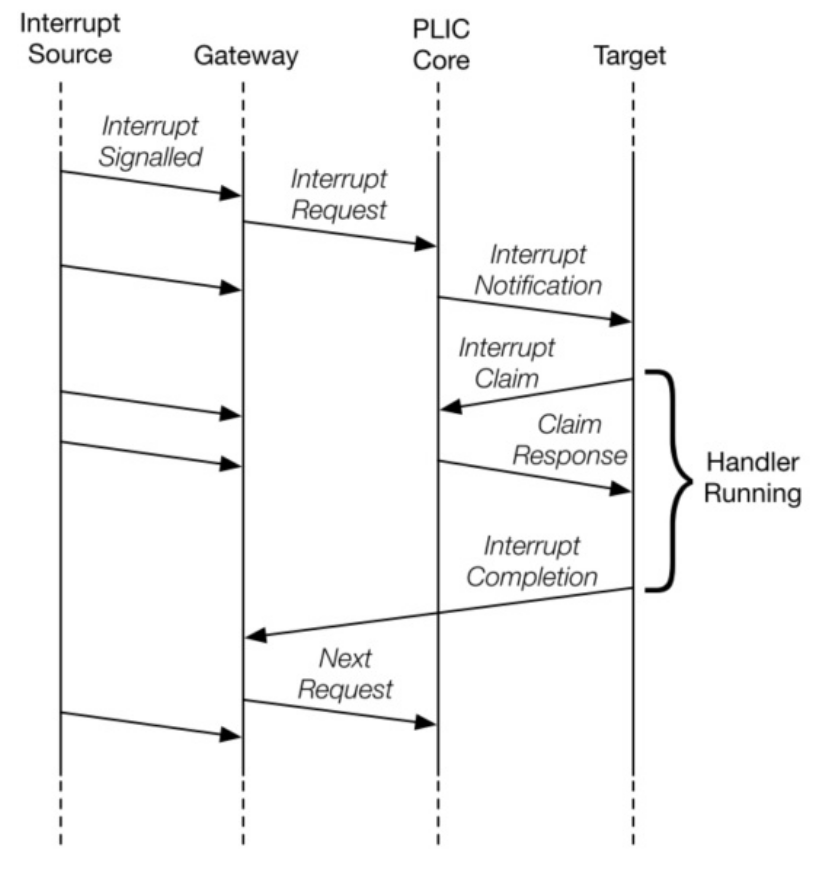
\includegraphics[width=0.7\textwidth]{plic_int_flow.png}
    \caption{\acrshort{plic} Interrupt Flow.}
    \label{fig:plic_int_flow}
\end{figure}

Table \ref{tab:plic_spec_regs} shows the memory mapped registers that the \textit{RISC-V} \acrshort{plic} specification defines. The \acrshort{plic} unit maps most registers into consecutive memory positions depending on their type. Every register in the \acrshort{plic} hardware has a width of 32-bit. Nevertheless, each claim/complete and priority threshold register has an address offset of 0x1000 from the previous register, as shown in table \ref{tab:plic_spec_regs}. The \acrshort{plic} core can have up to 1023 interrupt sources and 15871 targets. Consequently, there are a maximum of 1023 interrupt source priority registers; 32 interrupt pending bit registers; 507872 enable bits registers, and 15871 claim/complete and priority threshold registers. For each context, there are 32 enable bits registers. The interrupt source priority registers store the priority value of each \acrshort{plic} source. The interrupt pending bit registers indicates if there exists a pending interrupt request from the respective \acrshort{plic} sources. The hardware uses the enable bits registers to know for which targets an interrupt from a certain source is enabled. If a context has a priority threshold, an interrupt with a lower priority than the threshold will not be sent to the respective target. The claim/complete registers are used in the interrupt flow seen in figure \ref{fig:plic_int_flow}.

\begin{table}[!htb]
    \centering
    \begin{tabular}{|l|l|l|l|}
    \hline
    \textbf{Address} & \textbf{Width (bit)} & \textbf{Access}    & \textbf{Description}                              \\ \hline
    0x0              & 32                   & -                  & Reserved (interrupt source 0 does not exist)      \\ \hline
    0x4              & 32                   & WARL~\footnotemark & Interrupt source 1 priority                       \\ \hline
    ...              & ...                  & ...                & ...                                               \\ \hline
    0xFFC            & 32                   & WARL               & Interrupt source 1023 priority                    \\ \hline
    0x1000           & 32                   & R                  & Interrupt Pending bit 0-31                        \\ \hline
    ...              & ...                  & ...                & ...                                               \\ \hline
    0x107C           & 32                   & R                  & Interrupt Pending bit 992-1023                    \\ \hline
    0x2000           & 32                   & RW                 & Enable bits for sources 0-31 on context 0         \\ \hline
    ...              & ...                  & ...                & ...                                               \\ \hline
    0x207C           & 32                   & RW                 & Enable bits for sources 992-1023 on context 0     \\ \hline
    ...              & ...                  & ...                & ...                                               \\ \hline
    0x1F1FFC         & 32                   & RW                 & Enable bits for sources 992-1023 on context 15871 \\ \hline
    0x200000         & 32                   & WARL               & Priority threshold for context 0                  \\ \hline
    0x200004         & 32                   & RW                 & Claim/complete for context 0                      \\ \hline
    ...              & ...                  & ...                & ...                                               \\ \hline
    0x201000         & 32                   & WARL               & Priority threshold for context 1                  \\ \hline
    0x201004         & 32                   & RW                 & Claim/complete for context 1                      \\ \hline
    ...              & ...                  & ...                & ...                                               \\ \hline
    0x3FFF000        & 32                   & WARL               & Priority threshold for context 15871              \\ \hline
    0x3FFF004        & 32                   & RW                 & Claim/complete for context 15871                  \\ \hline
    \end{tabular}
    \caption{\acrshort{plic} registers compatible \textit{RISC-V} specification.}
    \label{tab:plic_spec_regs}
\end{table}

\footnotetext{write-any-read-legal fields store only legal values written by CSR writes.}

Lastly, it is essential to note that the \acrshort{plic} hardware only needs to generate the needed registers. The needed registers depend on the number of sources and the number of targets the \acrshort{plic} hardware has to support. Those values can be passed as parameters to the \acrshort{plic} unit when the developer instantiates it in the \acrlong{hdl}. Consequently, if the number of sources is 32, the \acrshort{plic} hardware should only create 32 interrupt source priority registers, not 1023. The \acrshort{plic} parameters can influence the number of resources the hardware utilises.

\subsection{Compatible UART/Serial Console}
\label{section:serial_console}
In the \textit{RISC-V} Platform Specification~\cite{riscv_platform_specification} it is defined that every embedded \acrfull{os} is required to have a \acrshort{uart} port implementation that is register-compatible with the industry standard \textit{UART16550}. The \textit{UART16550} already exists for a long time, it was released by \textit{National Semiconductor} in 1987, and is present and supported by a large number of software and hardware. The \textit{UART16550} is often used connected to an RS-232 interface. The \textit{IOb-SoC} supported development boards are connected through RS-232 to the computer.

Table \ref{tab:uart16550_regs} presents the \textit{UART16550} registers that are always accessible after the \acrshort{soc} resets. The \textit{UART16550} contains more registers that are discussed further ahead. The registers in table \ref{tab:uart16550_regs} may have the same address if one register can only be read and the other can only be wrote. The \textit{UART16550} only uses the 5 \acrlong{lsb} of a 32-bit address to address its registers.
\begin{table}[!ht]
    \centering
    \begin{tabular}{|l|l|l|l|l|}
    \hline
    \textbf{Name} & \textbf{Address} & \textbf{Width (bit)} & \textbf{Access} & \textbf{Description}                                                                    \\ \hline
    \acrlong{rbr} & 0                & 8                    & R               & Receiver FIFO output                                                                    \\ \hline
    \acrlong{thr} & 0                & 8                    & W               & Transmit FIFO input                                                                     \\ \hline
    \acrlong{ier} & 1                & 8                    & RW              & \begin{tabular}[c]{@{}l@{}}Enable/Mask interrupts\\  generated by the UART\end{tabular} \\ \hline
    \acrlong{iir} & 2                & 8                    & R               & Get interrupt information                                                               \\ \hline
    \acrlong{fcr} & 2                & 8                    & W               & Control FIFO options                                                                    \\ \hline
    \acrlong{lcr} & 3                & 8                    & RW              & Control connection                                                                      \\ \hline
    \acrlong{mcr} & 4                & 8                    & W               & Controls modem                                                                          \\ \hline
    \acrlong{lsr} & 5                & 8                    & R               & Status information                                                                      \\ \hline
    \acrlong{msr} & 6                & 8                    & R               & Modem Status                                                                            \\ \hline
    \end{tabular}
    \caption{Assessable \textit{\acrshort{uart}16550} registers by default.}
    \label{tab:uart16550_regs}
\end{table}

The \acrshort{rbr} and the \acrshort{thr} are the \textit{UART16550} registers the \acrshort{soc} uses to send and receive data through the serial interface. The hardware uses the \acrshort{ier} and the \acrshort{iir} to enable and identify the different types of interrupts that can be generated in \textit{UART16550}. The interrupts generated by the \textit{UART16550} are forward to a \acrshort{plic} unit. The hardware can use the \acrshort{fcr} to control the receiver and transmitter \acrshort{fifo}s. The \acrshort{lcr} is able alter the \textit{UART16550} serial interface configuration and the \acrshort{lsr} indicates the current status of the serial connection. Lastly, the \acrshort{mcr} allows transferring control signals to a modem connected to
the \acrshort{uart} and the \acrshort{msr} displays the current state of the modem control lines.

Additionally there exist two clock divisor registers that together form a 16-bit register, table \ref{tab:uart16550_divisor_regs} shows their properties. The \textit{UART16550} uses the divisor latches register to adapt the reading and writing cycles depending on the system clock frequency and the system baud rate. When initialising the \acrshort{uart} in firmware the value stored in the registers should be $\frac{systemFrequency}{16*BaudRate}$. On the \acrshort{soc} reset both registers have all bits set to '0' and the IO interface is disabled. The IO interface is enabled after the divisor latch \acrshort{LSB} is written. Therefore developers must set the \acrshort{MSB} first. Since the divisor latches address is the same as the receiver and transmitter registers to access the divisor latches developers have to set the 7th bit of \acrshort{lcr} to '1'. After setting the divisor latches the bit should be restored to '0' to restore access to the receiver and transmitter registers.

\begin{table}[!ht]
    \centering
    \begin{tabular}{|l|l|l|l|l|}
    \hline
    \textbf{Name}              & \textbf{Address} & \textbf{Width (bit)} & \textbf{Access} & \textbf{Description}                                                                      \\ \hline
    Divisor Latch Byte 1 (\acrshort{LSB}) & 0                & 8                    & RW              & \begin{tabular}[c]{@{}l@{}}The \acrlong{LSB}\\  of the divisor latch\end{tabular} \\ \hline
    Divisor Latch Byte 2 (\acrshort{MSB}) & 1                & 8                    & RW              & \begin{tabular}[c]{@{}l@{}}The \acrlong{MSB}\\  of the divisor latch\end{tabular} \\ \hline
    \end{tabular}
    \caption{Divisor latch \textit{\acrshort{uart}16550} registers.}
    \label{tab:uart16550_divisor_regs}
\end{table}

Finally when using 32-bit data bus interface, there are two additional registers for debugging. The first register address is 8 and the second is 12. Both registers are 8 bits and read only. Some of the registers presented in table \ref{tab:uart16550_regs} are not relevant for the development of this thesis project. Nevertheless, the reader can study more about them in the documentation of the \textit{\acrshort{uart}16550}~\cite{gorban2002uart}.

\subsection{Supervisor Binary Interface}
\label{subsection:sbi}
Talk OpenSBI!

\subsection{The Linux Boot Flow}
\label{subsection:linux_boot_flow}
What is a device tree?

\section{Open Source Verification tools}
\label{section:verification_tools}
Verification tools are ....

Other emulators are Trace-accurate, like Spike, and Cycle-accurate, for example, Verilator. 

https://www.sifive.com/blog/risc-v-qemu-part-1-privileged-isa-hifive1-virtio

\subsection{Hardware logic simulators}
It is important to have a good hardware simulation environment for testing purposes. Researchers take advantage of already existing and well-developed tools. Several simulation tools exist, most of which are proprietary, for example, \textit{xcelium} from \textit{Candence}. Its utilisation can increase the cost of a project significantly. In this thesis, we will use open-source, free-to-use verification tools. In specific, we will take advantage of \textit{Icarus Verilog}~\cite{williams2006icarus} and \textit{Verilator}~\cite{snyder2010verilator}. Although both tools are for verification, they serve different purposes due to their characteristics.

\begin{itemize}
    \item \textbf{\textit{Icarus Verilog}} is a Logic Simulator that uses Verilog or System-Verilog testbench to test the UUT (Unit Under Test). Unfortunately, its support for System-Verilog is limited, and some designs might not run in this simulator. \textit{Icarus Verilog} is also known as \textit{IVerilog}.
    
    After compiling the hardware design, \textit{IVerilog} outputs a file which can be run line by line to simulate the designed logic.
    
    \item \textbf{\textit{Verilator}} transforms the \textit{Verilog} \acrshort{hdl} designs into a \textit{C++} program that can be executed after being compiled. Using \textit{C++} to create a testbench allows calling the converted hardware program as a function of a normal \textit{C++} library. Executing the \textit{C++} testbench simulates the hardware initially described in \textit{Verilog}. While also allowing to make use of system calls easily. The testbench needed to run with Verilator is similar to the testbench in \textit{Verilog} used with \textit{IVerilog}.
\end{itemize}

\textbf{The biggest differences} are: \textit{Verilator} only represents logic signal as 1's or 0's, contrary to \textit{IVerilog} which also represents unknown values as X's; Since \textit{Verilator} ends up being a C++ program it is much faster to run the simulation than with \textit{IVerilog}; On another perspective \textit{Verilator} is slower than \textit{IVerilog} to interpret the hardware logic design.
As such, it is easier to use \textit{IVerilog} to detect errors in the design, but it is better to use \textit{Verilator} for more complex simulations.

\subsection{\textit{QEMU} Simulation}
\textit{QEMU}~\cite{bellard2005qemu} is an open-source machine emulator and virtualiser that allows running software and firmware, like operating systems, on many different devices and architecture using a personal computer. \textit{QEMU} is similar to \textit{VMware}~\cite{bugnion2012bringing} or \textit{VirtualBox}~\cite{oracle2015virtualbox}. \textit{VMware} and \textit{VirtualBox} allow the user to create virtual machines that simulate real hardware and execute an operating system. Developers can use \textit{QEMU} to run an operating system on virtual hardware.

\textit{QEMU} is considered a functional emulator; it translates the instructions that were supposed to run on the target architecture to instructions that run on the host CPU. The advantage of using a functional emulator like \textit{QEMU} is that it is way faster than the other emulation types. A functional emulator runs 100 million to > 1 billion instructions per second, while trace-accurate or cycle-accurate run 10 to 100 thousand instructions per second.

\textit{QEMU} can be used to emulate both 32-bit and 64-bit \textit{RISC-V} CPUs. \textit{QEMU} is ideal for testing user applications written to execute on a \textit{RISC-V} embedded system. User applications, contrary to the initial bootloaders, are platform-independent. In case of an application not running on a certain \acrshort{soc}, developers can use \textit{QEMU} to check if the problem is the application or the \acrshort{soc}. A user can emulate an operating system by compiling the firmware to be compatible with the \textit{QEMU} \enquote{virt} board. The \enquote{virt} is a board that does not replicate any actual hardware. However, the \textit{QEMU} developers designed this virtual hardware so the users could test the software even if there existed no hardware that could run it. To define which board the emulation is supposed to run in when calling \textit{QEMU}, the user should pass \textit{--machine virt} as an argument.
